\section{Silniki 3D}
Mnogość źródeł jednoznacznie wskazuje, że gałąź jest dojrzała i oczekiwać można równie obfitej puli dostępnych rozwiązań.
Jest to w pełni prawidłowe założenie.
Rynek jest na tyle obszerny, że początkowo trudno zorientować się kto stanowi grono odbiorców dla poszczególnych produktów.
Poniższa sekcja ma za zadanie przybliżyć rozwiązanie tego problemu.
\par
W celu dokonania klasyfikacji konieczne będzie przygotowanie listy charakterystyk na podstawie których przykłady zostaną porównane.
Wśród wielu możliwych do najważniejszych zaklasyfikować można cechy produktu stanowiące odpowiedzi na pytania takie jak:
\vspace{-0.5\topsep}
\begin{itemize}
    \setlength{\parskip}{5pt plus 0pt}
    \setlength{\itemsep}{5pt plus 5pt}
    \item Czy jest multiplatformowy?
    \item Na zasadach jakiej licencji jest dystrybuowany?
    \item Czy jest aktywnie rozwijany?
    \item Czy dostępna jest dokumentacja i przykłady wykorzystania?
    \item Czy kod źródłowy jest otwarty?
    \item Jakie przypadki użycia realizuje?
    \item Jak wygląda kwestia rozszerzalności?
    \item Jak przebiega integracja?
\end{itemize}
\vspace{-0.5\topsep}
Uzyskanie odpowiedzi pozwoli oszacować, które obszary branży pokryte są przez istniejące rozwiązania.
Dodatkowo, umożliwi dostrzeżenie nie tylko silnych stron, ale także nisz, które kryją w sobie potencjał i mogłyby skorzystać z ulepszeń.
\subsection{Biblioteki multiplatformowe}
Jedną z dwóch możliwości dystrybucji oprogramowania jest forma multiplatformowa.
W założeniu polega ona na stworzeniu jednego rozwiązania, dostępnego na co najmniej dwóch platformach.
Warto podkreślić, że chodzi tutaj o architekturę w której istnieje część wspólna \longpause w rozpatrywanym znaczeniu nie należy uwzględniać oprogramowania realizującego identyczne funkcje, ale za pomocą ponownej, natywnej implementacji.
\par
Wysokopoziomowy projekt zachowuję pewną prawidłowość i ma warstwowy charakter.
Obszar współdzielony tworzony jest w technologii dostępnej na każdej ze wspieranych platform.
Poniżej niego znajduje się strefa specyficzna dla systemu, która ma uwzględniać ewentualne różnice w interakcji z jego zasobami.
Opcjonalnie, ponad nimi usytuowany jest natywny interfejs, mający za zadanie poprawić przystępność \longpause programista systemu Android oczekiwał będzie API w formie biblioteki JAVA lub Kotlin, zaś twórca aplikacji iOS powinien otrzymać dostęp za pośrednictwem języków Swift czy Objective-C.
\begin{figure}
    \begin{center}
        \includegraphics[width=10cm]{images/multiplatform-architecture.png}
    \end{center}
    \caption{Demonstracja idei oprogramowania mulitplatformowego}
    \label{fig:multiplatform}
\end{figure}
\par
Głównym argumentem stojącym za budowaniem oprogramowania w sposób multiplatformowy jest chęć zwiększenia grona odbiorców.
Dla konsumenta technologii jest to niewątpliwa zaleta, natomiast narzuca to na twórców dodatkową prace związaną z koniecznością uwzględnienia wpływu poszczególnych zmian na wszystkie dostępne warianty.
\par
Wprowadzenie generalizacji wiąże się jednakże z narzutem wydajnościowym.
Każdy istniejący poziom abstrakcji przekłada się na większą ilość wywołań pomiędzy obiektami wewnątrz biblioteki.
Możliwe minimalizowanie zjawiska jest newraligczne, każda strata płynności wynikająca z wzmożonego nakładu obliczeń procesora implikować będzie konieczność obniżenia jakości grafiki celem utrzymania pożądanej prędkości animacji. 
\par
Kolejnym aspektem, który należy wziąć pod uwagę jest sposób integracji z natywnym środowiskiem.
Oznacza to określenie czy interfejs biblioteki dla końcowej platformy uwzględnia powszechnie przyjęte konwencje.
W idealnym przypadku użytkownik powinien być w stanie domyślić się klucza komunikacji na podstawie posiadanych doświadczeń, bez konieczności wspierania się dokumentacją. 
\subsubsection{Unity}
Najpopularniejszym silnikiem grafiki trójwymiarowej na platformie iOS jest Unity.
Stworzony został z myślą o produkcji gier wideo.
Dostępny jest na większości platform, zarówno mobilnych, jak i stacjonarnych, ale w głównej mierze przeznaczony jest do mniejszych projektów.
\par
Rozwiązanie należy zaliczyć do płatnych, choć rozwój aplikacji wykorzystującej technologię można rozpocząć bezpłatnie.
Użytkownik, który jednak poważnie myśli o wydaniu komercyjnie rentownej aplikacji szybko dostrzeże mnogość ograniczeń.
Do najpoważniejszych zaliczyć można brak możliwości zmiany ekranu ładowania aplikacji czy niemożność dostępu do kodu aplikacji silnika.
\par
Z drugiej strony Unity to twór kompletny \longpause pozwala na tworzenie w technologiach 2D, 3D, VR oraz AR.
Posiada zintegrowane moduły do obsługi fizyki, dźwięku, kontrolerów, sieci, analityki użycia, a także reklam.
\par
Choć rozwijany jest w języku C++ to użytkownik dokonuje interakcji za pomocą C\#.
W założeniach chodzi o to, aby silnik skompilować tylko raz, a każda modyfikacja, której pragnie dokonać w rozgrywce była błyskawiczna pod względem przyrostowego czasu budowy.
Mono \longpause framework wykorzystywany przez Unity w tym celu \longpause ma jednak pewne mankamenty.
Przede wszystkim użytkownicy narzekają na okazjonalne przycięcia w grach wynikające ze specyfiki zarządzania pamięcią.
Dziwić może także sama obecność C\#.
Unity deklaruje, że najlepiej odnajduje się na mobilnych platformach, ale język skryptowy nie pokrywa się z żadną wiodącą technologią ze świata smartfonów.
Na obronę jednak przyznać należy, że grę w unity można stworzyć bez znajomości platformy docelowej.
\par
Dodatkowo, Unity jest rozszerzalne. 
Dokonać można tego za pomocą pluginów występujących w dwóch formach.
Jest to odpowiednio plugin natywny dla zadanego systemu operacyjnego, albo zgeneralizowany oferujący funkcjonalność dla wielu platform.
\par
Pomimo, że Unity jest stale rozwijane to grafika wydaje się odstawać od konkurencji.
Podkreślić należy, że potok renderowania silnika jest konfigurowalny, więc jeśli jakość dla odbiorcy jest niezadowalający istnieje możliwość dokonania korekcji we własnym zakresie.
Otwiera to także możliwość stworzenia zupełnie unikalnego stylu graficznego, choć zaakceptować należy wysoki poziom wymaganej wiedzy do osiągnięcia tego celu.
\par
Sama dokumentacja stoi na wysokim poziomie.
Obfita jest w liczne przykładowe projekty i zawiera sugestie co do sposobu implementacji pewnych funkcjonalności w sposób zgodny z wizją autorów.
\par
Pierwotnie cała interakcja warstwy gry oraz silnika obsługiwana była za pomocą skryptów C\#.
Na przestrzeni lat rozwinięto jednak interfejs graficzny środowiska, a także dodano możliwość konfigurowania przebiegu rozgrywki za pomocą programowania wizualnego.
W założeniu podobne jest to nieco do schematów blokowych używanych w celu objaśniania algorytmów.
Koncept miał za zadanie otworzyć silnik na szersze grono odbiorców i zaoferować możliwość tworzenia gier osobom niebędącym zaznajomionym z programowaniem.
Pozornie pomysł może wydawać się oszczędzać czas i ułatwiać rozwój, mimo to grono osób nadal niechętnie korzysta z rozwiązania.
W głównej mierze podyktowane jest to bardzo kiepską przejrzystością zmian dokonanych przez użytkowników w systemach kontroli wersji.
Równie często przywoływany jest także argument wskazujący na trudność w odnajdywaniu się w logice stworzonej przy pomocy programowania wizualnego.
Równoważna implementacja w formie skryptu traktowana jest jako bardziej przejrzysta, a więc łatwiejsza do zrozumienia.
\par
Za minus można uznać narzut w kwestii wagi aplikacji.
Szablon pustego projektu wiąże się z koniecznością posiadania około 20 MB wolnej przestrzeni.
Natywny, pusty projekt iOS to zaledwie 1 MB.
Wydawać może się to nieistotne, jednak z uwagi na fakt, że aplikacje mobilne często pobierane są za pomocą transmisji komórkowej, a na jej efektywność wpływa wiele czynników, to naturalnie waga powinna być ograniczona do minimum.
\par
Pewną charakterystyką większości silników do gier, włącznie z Unity, jest zapewnianie użytkownikowi własnego środowiska programistycznego.
Dodać należy, że nie jest ono alternatywą dla preferowanego edytora.
Potrafi znacznie więcej niż asekurować w pisaniu skryptów.
Za jego pomocą importować można zasoby takie jak modele czy muzyka i określać zależności pomiędzy nimi a obiektami używanymi w algorytmach skryptowych. 
Oprogramowanie jest także kluczowe w momencie, kiedy przychodzi czas wygenerowania paczek dla platform docelowych. 
Tak jak wcześniej wspomniano \longpause twórca nie musi znać nawet podstaw programowania każdego ze wspieranych systemów.
Silnik gry jest w stanie za niego wykonać wszystkie pośrednie kroki i dostarczyć gotowy plik binarny, będący finalnym produktem, gotowym do uruchomienia.
W przypadku platformy iOS czy macOS oznacza to, że projekty w formacie natywnym dla XCode są ulotne i generowane na nowo przy każdym eksporcie z Unity.
\par
Opisany powyżej sposób rozwijania aplikacji sprawia, że niebywale trudno wykorzystać jest silniki graficzne tylko w wycinku funkcjonalności.
Dedykowane są one do obsłużenia całości aplikacji od interfejsu, po warstwę sieciową aż po interakcje z komponentami platformy jak kamera czy żyroskop.
O ile w przypadku produkcji gier podejście nie budzi zastrzeżeń, o tyle niebywale nierozsądne byłoby opierać całą aplikację użytkową o silnik tylko w celu skorzystania z jego możliwości renderowania.
\begin{figure}
    \begin{center}
        \includegraphics[width=10cm]{images/engines/unity/example-game.png}
    \end{center}
    \caption{Przykładowa gra stworzona w silniku Unity}
    \label{fig:unity-example-game}
\end{figure}

% \subsubsection{Godot}
% Reprezentuje wszystko za pomocą grafu sceny
% Posiada UI do tworzenia gry -- node'y, animacje
% Napisać, że jak chcemy interfejsować z silnikiem to trzeba pisać pluginy do godota
% Posiada visual scripting za pomocą bloków
% używa GDScript do skryptowania, można skryptować C sharp albo C++
% Napisać, że obecnie jest w wersji 4
% Napisać, że godot jest właściwie vulkan only
% działa na macos i apple silicon od wersji 3.3 -- ale wtedy opierało się to na opengl
% teraz gdy apple odeszło od opengl godot kompiluje swoje shadery z vulkan do metal
% Na ten moment nie jest to stabilne
% community driven
% https://godotengine.org/showcase
% https://itch.io/games/made-with-godot/platform-ios
% Napisz, że gier na iosa to w sumie jest mało
% \begin{figure}[H]
%     \begin{center}
%         \includegraphics[width=15cm]{images/engines/godot/editor.png}
%     \end{center}
%     \caption{Edytor treści w silniku Godot}
%     \label{fig:godot-editor}
% \end{figure}

% \subsubsection{Unreal Engine}
% low end devices
% small teams
% open source
% 5 procent od sprzedaży unita powyżej pewnej sumy gross
% good performance
% May be overwhelming for a single person
% Constant patches
% Visual programming may be difficult and less visible for merges
% Inefficient use of data

% " UE4 is not intended to visualise and manage the sheer number of weapons, armor, consumables, conversations, and so on, needed for an RPG."

% UE4 is well suited to bigger games, so think carefully if you're aiming for a smaller project -- various aspects could run slowly, from the editor itself to official support. Unity may be better suited to your needs if you're working on a small game or a mobile game.

% "UE4 comes with the background of being an engine for large AAA titles supporting tons of features for all kinds of advanced systems," Hazelight's Coulianos says. "Therefore the editor can run slow, and seem a bit overkill if you are making a very small and simple game -- for a phone, for example."

% not very popular in simulation/racing games
% super grafika
% good for large, complex game
% blueprints -- visual programming
%  lots of materials for learning
% \fig{images/engines/ue/blueprints.png}{Kreator tworzenia logiki w silniku Unreal Engine 4}{fig:ue-blueprint}

% \begin{figure}[H]
%     \begin{center}
%         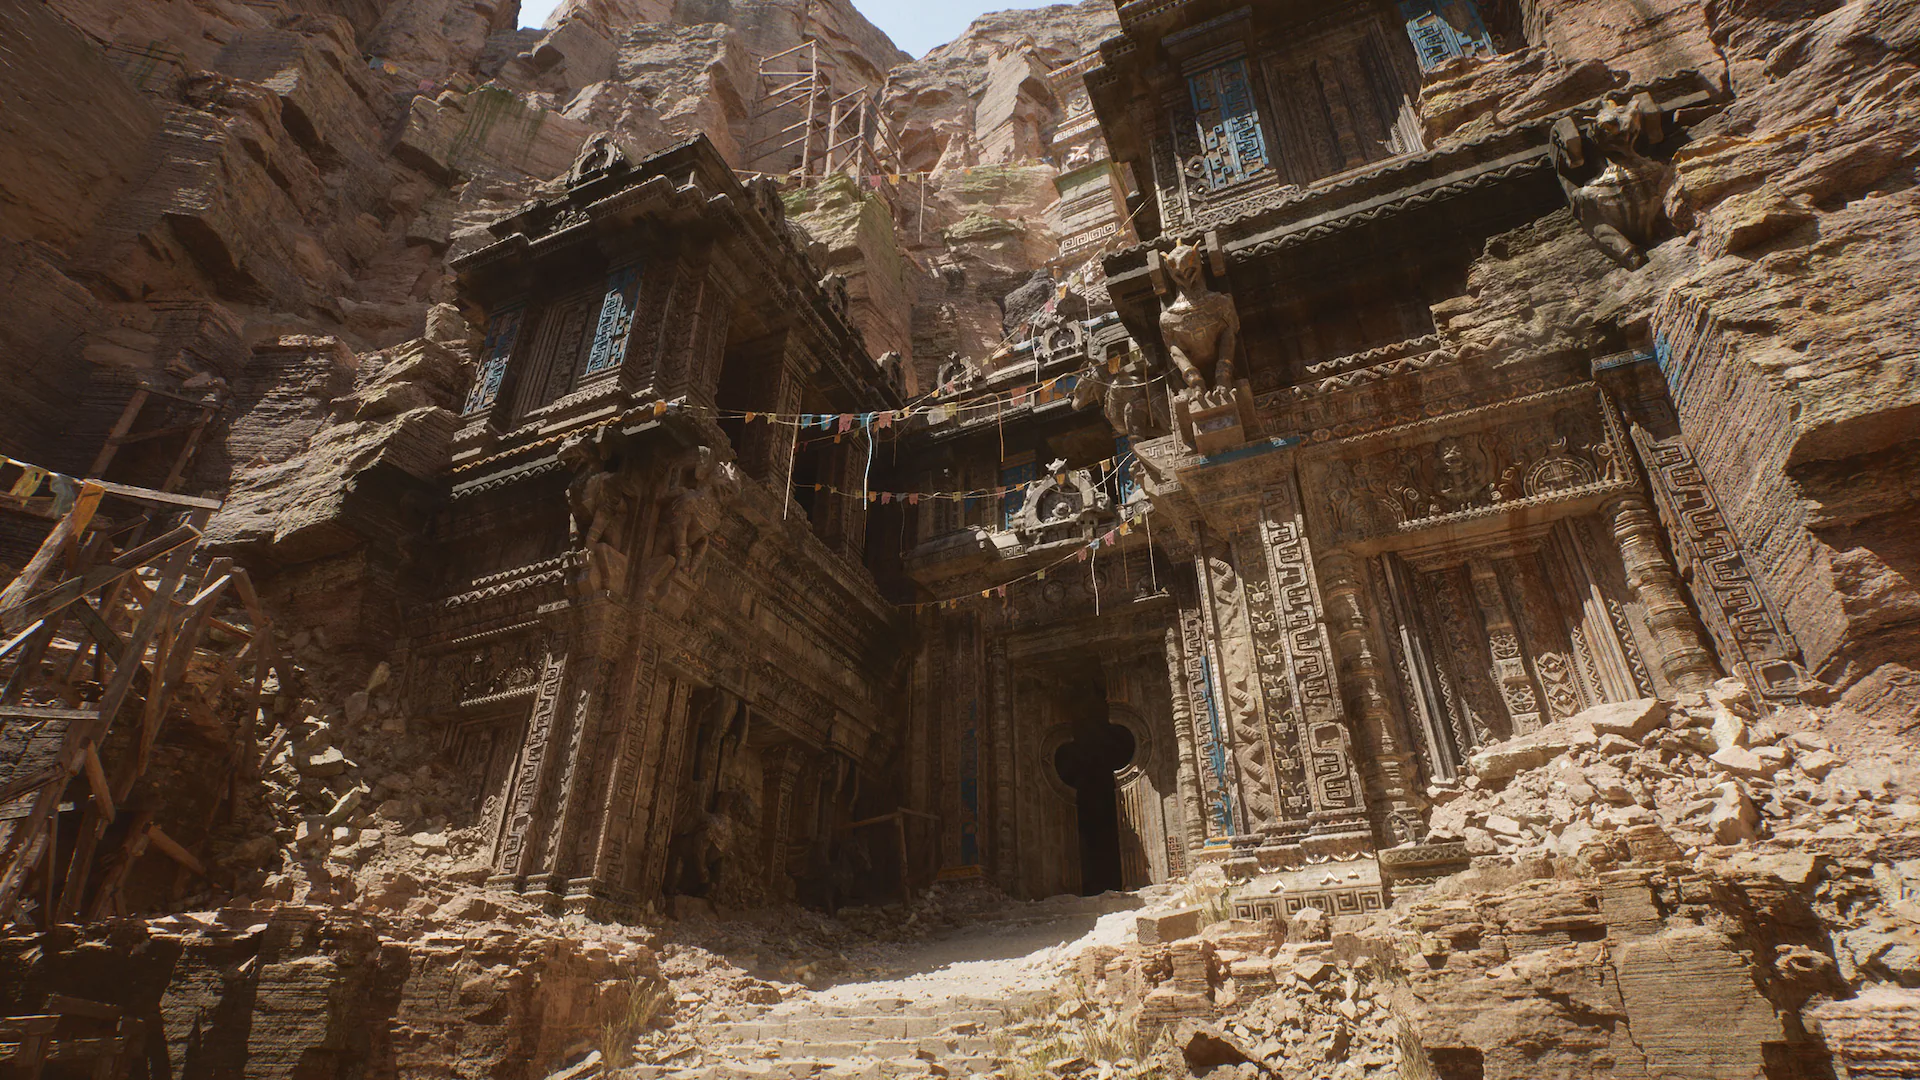
\includegraphics[width=15cm]{images/engines/ue/photorealistic-temple.png}
%     \end{center}
%     \caption{Przykład renderowania hybrydowego w Unreal Engine 5}
%     \label{fig:ue5-photorealistic-temple}
% \end{figure}

% \subsubsection{Filament}
% manual memory management
% good graphics, physically based,
% c++, based
% implies using objective-c in the project
% everything is written in c++
% \begin{figure}[H]
%     \begin{center}
%         \includegraphics[width=7cm]{images/engines/filament/helmet.jpeg}
%     \end{center}
%     \caption{Przykład klatki wygenerowanej przez silnik Filament}
%     \label{fig:filament-helmet}
% \end{figure}

\subsection{Biblioteki natywne}
Alternatywą do multiplatformowych rozwiązań są biblioteki natywne.
Włączyć do tej grupy można produkty dostępne tylko i wyłącznie na pojedynczym systemie lub te obecne na wielu, lecz posiadające wszystkie warianty zbudowane od podstaw.
Pomimo, że wsparcie każdego środowiska z osobna może postrzegane być jako nieuzasadniona aprobata powtarzalności to przynosi ono także korzyści.
\par
Jedną z najważniejszych zalet jest możliwość osiągnięcia optymalnej wydajności.
Kod źródłowy dostosowany pod konkretną platformę nie musi posiadać szeregu dodatkowych warstw.
\par
Natywność to również większa intuicyjność, wynikającą z możliwości tworzenia interfejsu dostosowanego do przyjętych konwencji.
Pojęcie jest ogólne, składa się na nie nazewnictwo, schemat komunikacji czy hermetyzacja.
\par
Aplikacja spójna technologicznie zyskuje też w sytuacji analizy potencjalnych problemów.
W przypadku otwartego kodu źródłowego przyczynić może się to do wzrostu kontrybucji ze strony społeczności.
\subsubsection{SceneKit}
\begin{figure}
    \begin{center}
        \includegraphics[width=15cm]{images/engines/scene-kit/editor.jpg}
    \end{center}
    \caption{Edytor treści w silniku SceneKit}
    \label{fig:scenekit-editor}
\end{figure}

\begin{figure}
    \begin{center}
        \includegraphics[width=15cm]{images/engines/scene-kit/example-game.jpg}
    \end{center}
    \caption{Przykładowa gra w silniku SceneKit}
    \label{fig:scenekit-example-game}
\end{figure}
Debiut rozwiązania nastąpił w 2012 roku. 
Za projekt i wykonanie odpowiedzialna jest firma Apple, której urządzenia stanowią jedyną docelową grupę odbiorców oprogramowania.
Początkowo wsparcie ograniczało się do platformy OS X, rozszerzenie dostępności na urządzenia mobilne nadeszło w 2014 roku, a na przestrzeni lat objęło również watchOS oraz tvOS.
\par
Pragnąc zaklasyfikować SceneKit najtrafniej byłoby określić, iż jest to biblioteka graficzna realizująca dodatkowo pewne funkcjonalności silnika do gier.
Jest to możliwość kontroli audio oraz integracja modelu fizycznego, będącego w stanie symulować wzajemny wpływ obiektów. 
W przeciwieństwie do wiodących rozwiązań skierowanych do branży gier SceneKit nie posiada własnego IDE, nie pozwala na programowanie wizualne, ani zaawansowane skryptowanie.
\par
Myśląc o grupie docelowej wskazać można deweloperów tworzących gry typu indie \longpause w niewielkiej grupie, z małym budżetem.
Ponadto, SceneKit świetnie sprawdza się w roli generatora grafiki trójwymiarowej w aplikacjach innych niż gry wideo.
Z uwagi na fakt, że jest to technologia natywna bardzo łatwo wkomponować można widoki z animowanymi scenami w aplikacje pełniącą inną funkcje niż rozrywkowa.
\par
Narzut użycia biblioteki na wielkość paczki jest niewielki.
W pesymistycznym przypadku wzrost wagi wynieść może 4 MB, jednak potencjalne usunięcie nieużywanych symboli przełoży się na znaczną redukcje tej wartości.
\par
Nie bez przyczyny wspomniano o dacie wydania biblioteki.
Choć jej interfejs ewoluował i rozrastał się w miarę upływu lat to założenia pozostały niezmienione.
2015 był rokiem kiedy podczas konferencji WWDC Apple zaprezentowało koncepcje, które sugerowały programistom wykorzystującym język Swift podejście oparte o komunikacje zorganizowaną wokół protokołów.
W głównej mierze uogólnić można je na zestaw sugestii, które sprawią, że kod będzie reużywalny, testowalny oraz przejrzysty.
Producent stopniowo wcielał je w swoje biblioteki, podczas uaktualniania języka Swift.
Niestety reforma ta nie dotknęła SceneKit, który współcześnie postrzegany jest już jako przestarzały.
\par
2018 rok był ostatnim kiedy wprowadzono usprawnienia do produktu.
Od tamtego czasu użytkownicy nie otrzymali żadnych poprawek, ani stanowiska Apple wyjaśniającego przyszłość projektu.
Sytuację komplikuje fakt, że kod źródłowy jest zamknięty, więc nie istnieje szansa rozwoju na własną rękę.
\par
Pomimo, że Apple jest gigantem, ma ogromne dochody i przez wielu programistów traktowane jest jako miejsce w którym jakość jest najważniejsza, to nadal w pewnych kwestiach można poczuć się zawiedzionym.
Jedną z takich chwil jest spojrzenie na dokumentację SceneKit.
Przyznać należy, że w sieci dostępnych jest wiele projektów demonstrujących działanie.
Natomiast pozytywny obraz przyćmiewają wszechobecne lakoniczne opisy odnoszące się do zawartości biblioteki.
Niejednokrotnie klasy oraz ich zmienne posiadają wyjaśnienia w formie pojedynczych zdań, nie nadających im szerszego kontekstu.
Odnieść można wrażenie, że jedyną drogą do zrozumienia pewnej puli z zaimplementowanych mechanizmów będzie wysnucie własnych wniosków empirycznie.
\subsubsection{ARKit}
Wydanie ARKit było odpowiedzią na rosnące zainteresowanie branży technologią rozszerzonej rzeczywistości.
Idea polega na wzbogacaniu obrazu przechwytywanego z kamery urządzenia o dodatkowe elementy 2D oraz 3D.
Podobnie jak w przypadku SceneKit jest to autorska biblioteka Apple.
Choć część funkcjonalności wydaje się być współdzielona jest z SceneKit to firma deklaruje, iż rozwiązania nie są w żadnym stopniu powiązane ze sobą.
\par
ARKit poprawia wiele problemów, które obecne są w SceneKit.
Przede wszystkim jest ona aktywnie rozwijana, na bieżąco publikowane są poprawki, rozszerzenia funkcjonalności i ulepszenia modelu oświetlenia.
\par
Interfejs ARKit jest kolejnym czynnikiem zaskakującym pozytywnie.
Dostosowany jest do współczesnych konwencji firmy i dobrze integruje się z resztą systemu.
Tak jak wspomniano wcześniej interakcje oparte o luźne powiązania pozytywnie wpływają na testowalność kodu wykorzystującego bibliotekę.
\par
Podobnie jednak jak w przypadku innych rozwiązań Apple ARKit nie jest otwarty.
Nie istnieje możliwość wglądu do kodu, ani jego modyfikacji, technologia może być jednak w nieodpłatny sposób wykorzystana z uwzględnieniem przeznaczenia do celów komercyjnych.
\begin{figure}
    \begin{center}
        \includegraphics[width=15cm]{images/engines/ar-kit/example-app.jpg}
    \end{center}
    \caption{Rzeczywistość rozszerzona na przykładzie aplikacji mobilnej}
    \label{fig:arkit-example-app}
\end{figure}
\par
Inteligentne suplementowanie obrazu obarczone jest jednak niemałym kosztem.
Każda klatka analizowana jest pod kątem semantyki, a ewentualny ruch wpływający na generowane obiekty rozszerzonej rzeczywistości kompensowany.
Spodziewać należy się, że mimo budzącego podziw modelu oświetlenia wydajność będzie przeciętna.
\par
Zaskakiwać może, że ARKit obsługuje jedynie iOS.
Na pozostałych platformach nie występuje lub tak jak przypadku międzyplatformowej technologii \textit{mac catalyst} wywołania są ignorowane.
Z jednej strony to zrozumiałe, ponieważ tylko telefony i tablety posiadają stosowne kamery spełniające wymagania.
Z drugiej wyklucza to możliwość wykorzystania ARKit do użycia w celu wygenerowania prostych scen 3D bez AR.
\subsection{Pozostałe silniki}
W celu dokonania rzetelnej oceny rynku dokonano także przeglądu projektów open source udostępnionych za pomocą platform github.com oraz gitlab.com.
Kryterium, którego spełnienia oczekiwano była dostępność na wszystkie platformy Apple i możliwość uruchomienia biblioteki na najnowszych systemach operacyjnych.
W rezultacie wyszukiwania znaleziono około dziesięciu projektów, niestety żaden z nich nie mógł określony być jako stabilne rozwiązanie do zastosowania produkcyjnego.
Do będących w stosunkowo zaawansowanej formie rozwoju zaliczyć można Satin~\cite{satin_project} oraz SwiftVVD~\cite{swiftvvd_project}.
% Powinienem pokusić się o napisanie czegoś więcej
\par
Warto wspomnieć, że poza wymienionymi przykładami bibliotek oraz silników istnieje wiele innych alternatyw.
Jako najpopularniejsze można przytoczyć tutaj jmonkey, urho3d, OGRE 3D, Amazon Lumberyard czy panda 3d.
Wszystkie z nich oparte są o podejście open-source.
Były to rozwiązania niegdyś popularne lub stale zwiększające swoje zasięgi, jednak ze względu na koncentrację pracy wokół całego ekosystemu Apple wyłączono je z dalszej analizy.
Głównie za sprawą skierowania jedynie na platformy stacjonarne lub wybrakowane wsparcie spowodowane zamknięciem się firmy Apple na API inne niż Metal.
\par
Sytuacja podobnie wygląda w przypadku silników na potrzeby gier AAA, takich jak CryEngine, Frostbite, RAGE czy Naughty Dog Game Engine.
Wszystkie z nich cieszą się niemałą popularnością i sukcesem w świecie gier.
Niestety są one skierowane tylko i wyłącznie na stacjonarne platformy.
Dodatkowo, część podlega opłatom licencyjnym, zaś inne nie mogą być w ogóle użyte z uwagi na fakt, że ich źródła są niepubliczne, a pliki binarne dystrybuowane są jedynie do projektów na potrzeby firm posiadających prawa autorskie.
